\documentclass[portrait,a0,final]{a0poster}

\usepackage{multicol}
\usepackage{color, colortbl}

\usepackage{graphicx}
\usepackage{color, colortbl}
\usepackage{fancyhdr}
\usepackage{epstopdf}
\epstopdfsetup{update}
\usepackage{pgfplots}
\usepackage[group-separator={,}]{siunitx}
\usepackage{fancyref}
\usepackage{algorithm}
\usepackage{algpseudocode}
\usepackage{url}
\usepackage[shortcuts]{extdash}
\usepackage{enumitem}
\usepackage{amssymb}
\usepackage{authblk}
\usepackage{tcolorbox}
\usepackage{lettrine}

\pagestyle{fancy}
\pagenumbering{gobble}
\definecolor{gray}{gray}{0.97}

\tcbset{size=fbox,colframe=black,colback=white,outer arc=0pt,arc=0pt,boxrule=3pt,boxsep=20pt,fonttitle=\Large}

\DeclareSIUnit{\btc}{BTC}
\DeclareSIUnit{\ghash}{GHash}
\DeclareSIUnit{\block}{block}
\sisetup{
  per-mode = symbol,
  inter-unit-product = \ensuremath{{}\cdot{}},
  parse-numbers=false
}

\begin{document}

\setlength{\columnsep}{50pt}

\title{\veryHuge Approximate Bitcoin Mining}
\author{\Large Matthew Vilim, Henry Duwe, Rakesh Kumar}
\affil{\Large Department of Electrical and Computer Engineering, University of Illinois at Urbana-Champaign}
\date{}
\maketitle

\begin{multicols}{3}

\begin{tcolorbox}[title=Abstract]
\lettrine{B}{itcoin} is the most popular cryptocurrency today. A bedrock of the Bitcoin framework is \emph{mining}, a computation intensive process that is used to verify Bitcoin transactions for profit. We observe that mining is inherently error tolerant due to its embarrassingly parallel and probabilistic nature. We exploit this inherent tolerance to inaccuracy by proposing approximate mining circuits that trade off reliability with area and delay. These circuits can then be operated at Better Than Worst-Case (BTWC) to enable further gains. Our results show that \emph{approximation} has the potential to increase mining profits by 30\%.
\end{tcolorbox}

\begin{tcolorbox}[title=Mining Background]
\lettrine{T}{he} Bitcoin mining process is summarized in Figure \ref{mining_process}. Mining consists of searching for a cryptographic \emph{nonce} value within a block such that the hash of the block falls within a certain range.
\end{tcolorbox}

\begin{figure}[H]
\caption{Compilation Flow}
\label{fig:flow}
\centering
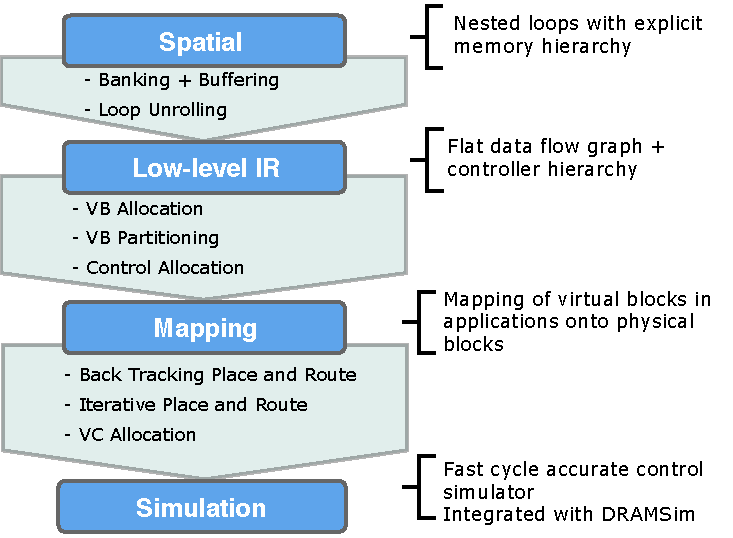
\includegraphics[width=1\linewidth]{figs/flow.pdf}
\end{figure}

\begin{figure}[H]
\caption{Mapping Application onto Plasticine}
\label{fig:mapping}
\centering
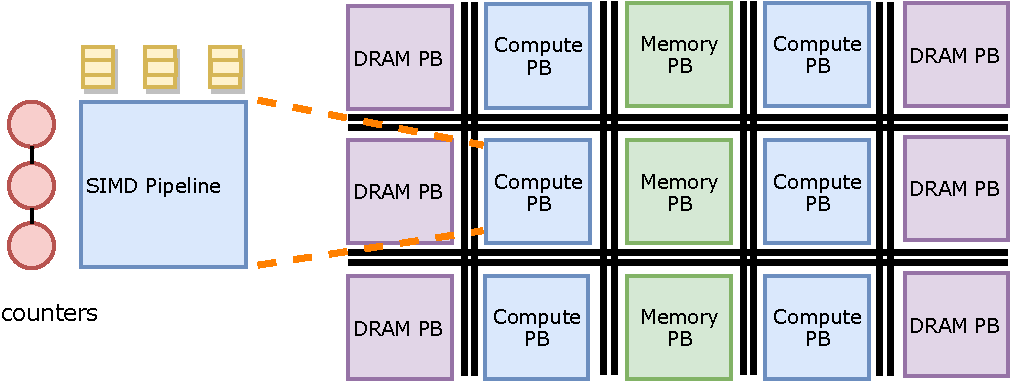
\includegraphics[width=1\linewidth]{figs/arch.pdf}
\end{figure}

\begin{figure}[H]
\caption{Graph characteristic for spatial applications}
\label{fig:link}
\centering
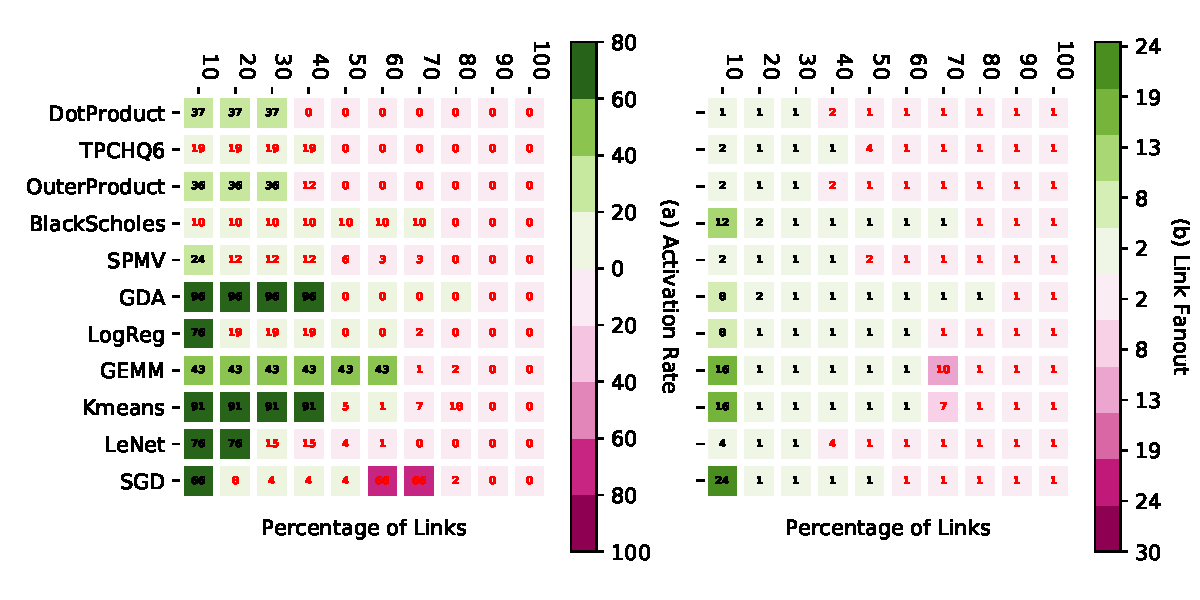
\includegraphics[width=1\linewidth]{figs/link5.pdf}
\end{figure}

\begin{figure}[H]
\caption{Area overheads for network architectures}
\label{fig:area}
\centering
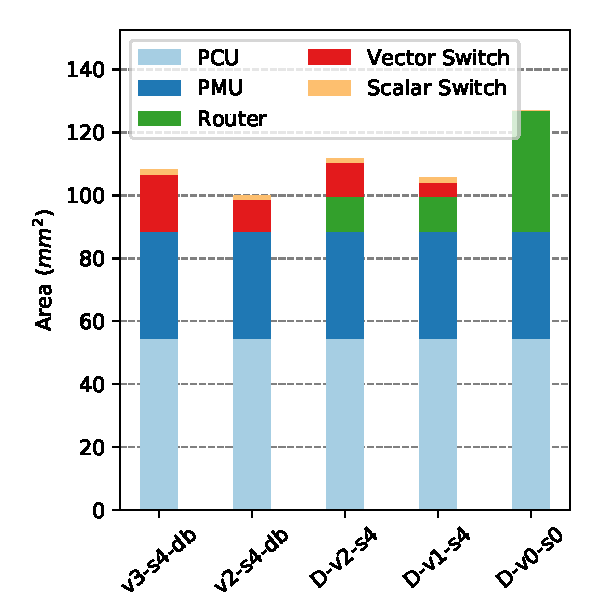
\includegraphics[width=1\linewidth]{figs/area.pdf}
\end{figure}

\begin{tcolorbox}
\lettrine{T}{he} mining algorithm is shown in Algorithm \ref{alg:mining_process}. In short, mining is a search for the nonce value that results in a double SHA-256 hash $digest$ (Algorithm \ref{alg:sha256}) value less than a given \emph{threshold}. The nonce is a 32-bit field within a 1024-bit \emph{block header}. In order to verify transactions at a steady rate, this threshold varies over time as a function of difficulty $D(t)$. Difficulty is adjusted by the network regularly such that a solution is expected to be found approximately every 10 minutes, regardless of the network's collective hash rate.
\end{tcolorbox}

\hfill
\begin{algorithm}[H]
\caption{Mining Process}
\label{alg:mining_process}
\begin{algorithmic}[1]
\State $nonce\gets 0$
\While{{$nonce < 2^{32}$}}
\State $threshold \gets ((2^{16} - 1) \ll 208) / D(t)$
\State $digest \gets$ SHA-256(SHA-256($header$))
\If {digest $< threshold$}
\State \Return $nonce$
\Else
\State $nonce \gets nonce + 1$
\EndIf
\EndWhile
\end{algorithmic}
\end{algorithm}

\begin{tcolorbox}[title=SHA-256 Datapath Overview]
\lettrine{F}{or} our studies, we selected as baseline the SHA-256 ASIC design outlined by Dadda et al. A summary of SHA-256 is provided in Algorithm \ref{alg:sha256}. The hashing core in this design is implemented as two parallel pipelines, the Compressor (Line \ref{alg:line:compress} of Algorithm \ref{alg:sha256}) and the Expander (Line \ref{alg:line:expand} of Algorithm \ref{alg:sha256}) shown in Figure \ref{fig:sha256_datapath}.

\label{alg:sha256}
\begin{itemize}
\item The message $M$ is divided into $N$ 512-bit blocks \\ $M^{(0)}, M^{(1)},\ldots,M^{(N-1)}$. Each of these blocks is further subdivided into 16 32-bit words $M^{(i)}_0, M^{(i)}_1,\ldots,M^{(i)}_{15}$.
\item The intermediate hash value $H^{(i)}$ is composed of 8 32-bit words $H^{(i)}_0, H^{(i)}_1,\ldots,H^{(i)}_{7}$.
\item $Ch(x,y,z) \equiv (x \land y) \oplus (\neg x \land z)$
\item $Maj(x,y,z) \equiv (x \land y) \oplus (x \land z) \oplus (y \land z)$
\item $\Sigma_0(x) \equiv x \ggg 2 \oplus x \ggg 13 \oplus x \ggg 22$
\item $\Sigma_1(x) \equiv x \ggg 6 \oplus x \ggg 11 \oplus x \ggg 25$
\item $\sigma_0(x) \equiv x \ggg 7 \oplus x \ggg 18 \oplus x \gg 3$
\item $\sigma_1(x) \equiv x \ggg 17 \oplus x \ggg 19 \oplus x \gg 10$
\end{itemize}
\end{tcolorbox}

\hfill
\begin{algorithm}[H]
\caption{SHA-256}
\label{alg:sha256}
\begin{algorithmic}[1]
\Function{SHA-256}{M}

\For{$i$ from $0$ to $N - 1$}
\For{$j$ from 0 to 15} \label{alg:line:expand}
\State $W_j = M^{(i)}_j$
\EndFor
\For{$j$ from 16 to 63}
\State $W_j = \sigma_1(W_{j-2}) + W_{j-7} + \sigma_0(W_{j-15}) + W_{j-16}$
\EndFor

\Statex
\For{$j$ from 0 to 63} \label{alg:line:compress}
\State $t_0 \gets h + \Sigma_1(e) + Ch(e,f,g) + K_j + W_j$
\State $t_1 \gets \Sigma_0(a) + Maj(a,b,c)$
\State $h \gets g$; $g \gets f$
\State $f \gets e$; $e \gets d + t_1$
\State $d \gets c$; $c \gets b$
\State $b \gets a$; $a \gets t_1 + t_2$
\Statex
\State $H^{(i)}_0 \gets H^{(i-1)}_0 + a$; $H^{(i)}_1 \gets H^{(i-1)}_1 + b$
\State $H^{(i)}_2 \gets H^{(i-1)}_2 + c$; $H^{(i)}_3 \gets H^{(i-1)}_3 + d$
\State $H^{(i)}_4 \gets H^{(i-1)}_4 + e$; $H^{(i)}_5 \gets H^{(i-1)}_5 + f$
\State $H^{(i)}_6 \gets H^{(i-1)}_6 + g$; $H^{(i)}_7 \gets H^{(i-1)}_7 + h$
\EndFor
\EndFor
\State \Return $H^{(N-1)}$
\EndFunction
\end{algorithmic}
\end{algorithm}

\hfill

\begin{tcolorbox}[title=Approximate Mining]
\lettrine{A}{} miner's instantaneous profit $p(t,f)$ at time $t$ and frequency $f$ is a function of the mining yield $Y(t)$ (\si{USD \per GHash}), hash rate $H(f)$ (\si{GHash\per\second}), power consumption $P(f)$ (\si{\kilo\watt}), and cost of electricity $C_e(t)$ (\si{USD\per\kWh}).

\begin{equation}
\label{eq:profit}
p(t,f) = H(f) \cdot Y(t) - P(f) \cdot \frac{C_e(t)}{60 \cdot 60}
\end{equation}

\lettrine{I}{n} the presence of approximation, the effective hash rate changes. A fraction $E(f)$ (error rate) of the computed hashes will be incorrect, and a normalized reduction in area $\hat{A}$ may occur.

\begin{equation}
\label{eq:hash_rate}
\tilde{H}(f) = \frac{1 - E(f)}{\hat{A}} \cdot H(f)
\end{equation}

\lettrine{T}{here} are $64 \cdot 3 = 192$ additions in a single round of SHA-256, each with error rate $E_{CPA}$. The error rate of a single round in the hashing core, therefore, is:

\begin{equation}
\label{eq:error_func}
E_f = 1 - (1 - E_{CPA})^{192}
\end{equation}

\lettrine{T}{he} error rate at each operating point is found through simulation. Each simulated SHA-256 round has error rate $E_i(f)$, the sum of functional and operational error rates. Bitcoin requires two rounds for each nonce iteration; hence, we can extrapolate to calculate cumulative error rate $E(f)$, assuming the hash inputs and outputs to be uniform random variables.

\begin{equation}
E_i(f) = E_f + E_o(f) \qquad E(f) = 1 - [1 - E_i(f)]^2
\end{equation}
\end{tcolorbox}

\begin{tcolorbox}[title=Results]
\lettrine{T}{able} \ref{table:adders} lists the adders' delay and area. Each adder was inserted into the hashing core pipelines in the CPA slots indicated in Figure \ref{fig:sha256_datapath}. The resulting hashing core area and delay are provided in Table \ref{table:pipeline}. Approximate variants are highlighted in gray. Figure \ref{fig:freq_scaling} shows the error rate-frequency characteristic $E_i(f)$ of each hashing core for various adders after simulating a full round of SHA-256. The resulting frequency-profit relation is shown in Figure \ref{fig:profit_freq}.
\end{tcolorbox}

\begin{table}[H]
\centering
\caption{Adder Comparison}
\label{table:adders}
\begin{tabular}{l*{5}{c}r}
Adder & delay $\cdot$ area (\si{\nano\second \cdot {\micro\meter}^2}) & P (\si{\milli\watt}) & $E_{CPA}$ \\
\hline
RCA & 7116 & 0.170 & NA \\
CLA & 4834 & 0.889 & NA \\
\rowcolor{gray}
GDA\textsubscript{(1,4)} & 3558 & 0.950 & $1.90 \times 10^{-5}$ \\
KSA\textsubscript{32} & 3631 & 0.867 & NA \\
\rowcolor{gray}
KSA\textsubscript{16} & 2862 & 0.814 & $4.60 \times 10^{-5}$ \\
\rowcolor{gray}
KSA\textsubscript{8} & 2102 & 0.715 & $2.26 \times 10^{-2}$ \\
\end{tabular}

\centering
\caption{Hashing Core Comparison for Different Adder Choices}
\label{table:pipeline}
\begin{tabular}{l*{4}{c}r}
Adder & delay $\cdot$ area (\si{\nano\second \cdot {\micro\meter}^2}) & P (\si{\milli\watt}) & $E_f$ \\
\hline
RCA & 210,0597 & 7.19 & NA \\
CLA & 123,865 & 12.1 & NA \\
\rowcolor{gray}
GDA\textsubscript{(1,4)} & 108,207 & 13.8 & $7.27 \times 10^-3$ \\
KSA\textsubscript{32} & 90,769 & 17.33 &  NA \\
\rowcolor{gray}
KSA\textsubscript{16} & 82,744 & 19.0 & $8.79 \times 10^{-2}$ \\
\rowcolor{gray}
KSA\textsubscript{8} & 73,152 & 20.4 & $1.00$ \\
\end{tabular}
\end{table}

\begin{tcolorbox}[title=Conclusions]
\lettrine{M}{ining} is a particularly good candidate for approximation because hashes are computed independently and in parallel, mitigating the effect of errors, and a built-in verification system detects any false positives. Furthermore, we have identified adders as beneficial choices for approximation in hashing cores in a mining ASIC. However, not all approximate adders yield increases in profit. Profits are maximized by adders that minimize delay at the expense of area, and approximate adders should be chosen accordingly. Moreover, profits may be improved by operating the hashing cores at Better Than Worst-Case (BTWC) operating points, past their nominal frequencies.
\end{tcolorbox}

\end{multicols}

%\includegraphics[width=0.15\linewidth]{ilogo_horz_bw}

\end{document}
